\section{První týden}

\subsection{Důkaz souvislosti minima a maxima}

Tvrzení:

pro $f: D \rightarrow \R, M \subseteq D, \hat{x} \in M$ platí:

\begin{enumerate}[(1)]
    \item $\hat{x} \in \underset{x \in M}{\argmin} f(x) \iff \hat{x} \in \underset{x \in M}{\argmax} (-f(x))$,
    \item jesliže $\hat{x} \in \underset{x \in M}{\argmin} f(x)$, pak $\underset{x \in M}{\min} f(x) = 
    - \underset{x \in M}{\max} (-f(x))$.
\end{enumerate}

(1) $\hat{x} \in \underset{x \in M}{\argmin} f(x)$, tj. $f(\hat{x}) \leq f(x), \forall x \in M \underset{\cdot (-1)}{\iff} 
-f(\hat{x}) \geq -f(x), \forall x \in M$, tj. $\hat{x} \in \underset{x \in M}{\argmax} (-f(x)). \qed$


(2) Ať $\hat{x} \in \underset{x \in M}{\argmin} f(x)$, pak $\underset{x \in M}{\min} f(x) = f(\hat{x}) = 
- (- f(\hat{x})) \overset{(1)}{=} - \underset{x \in M}{\max} (-f(x)). \qed$

\subsection{Hledání přípustných množin}
\begin{align*}
    \text{minimalizujte } x^2 + 1 \\
    \text{za podmínek } \frac{3}{x} \leq 1, \\
    x \in \N.
\end{align*}
Upravíme podmínky a uděláme jejich průnik: $x - 3 \geq 0 \land x \in \N \Rightarrow M = \N \setminus \bc{1,2}$.

Úvahou pak lze uhodnout minimum - minimum leží v bodě $x=3$.

\subsection{Hledání přípustných množin}
\begin{align*}
    \text{maximalizujte } \ln x \\
    \text{za podmínek } x \leq 5, \\
    \cos(\pi x) = 1.
\end{align*}
$D(f) = (0, \infty)$. 

Udělejme průnik definičního oboru funkce a podmínek: $x \in (0, \infty) \land x \leq 5 \land \cos(\pi x)=1$.

\begin{multicols}{2}
    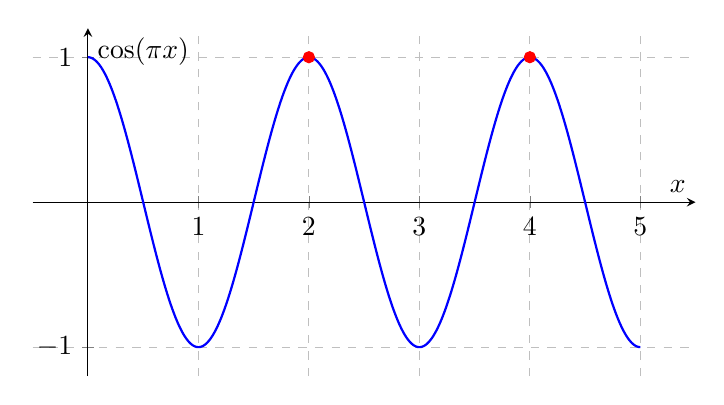
\begin{tikzpicture}
        \begin{axis}[
            axis lines = middle,
            xlabel = $x$,
            ylabel = {$\cos(\pi x)$},
            domain=0:5,
            samples=1000,
            %   xtick={0,1,2,3,4,5},
            %   ytick={-1,-0.5,0,0.5,1},
            enlargelimits,
            grid=both,
            minor grid style={dotted},
            major grid style={dashed},
            width=10cm, height=6cm,
        ]
            \addplot[blue, thick] {cos(deg(x * pi))};
            \addplot[only marks, red, mark=*] coordinates {(2,1) (4,1)};
        \end{axis}
      \end{tikzpicture}
\columnbreak

      \quad Očividně tedy $M = \bc{2,4}$.

      \quad Úvahou pak lze uhodnout $\underset{x \in M}{\argmax} \ln x = \bc{4}$.
\end{multicols}
